% Options for packages loaded elsewhere
\PassOptionsToPackage{unicode}{hyperref}
\PassOptionsToPackage{hyphens}{url}
%
\documentclass[
]{article}
\usepackage{amsmath,amssymb}
\usepackage{iftex}
\ifPDFTeX
  \usepackage[T1]{fontenc}
  \usepackage[utf8]{inputenc}
  \usepackage{textcomp} % provide euro and other symbols
\else % if luatex or xetex
  \usepackage{unicode-math} % this also loads fontspec
  \defaultfontfeatures{Scale=MatchLowercase}
  \defaultfontfeatures[\rmfamily]{Ligatures=TeX,Scale=1}
\fi
\usepackage{lmodern}
\ifPDFTeX\else
  % xetex/luatex font selection
\fi
% Use upquote if available, for straight quotes in verbatim environments
\IfFileExists{upquote.sty}{\usepackage{upquote}}{}
\IfFileExists{microtype.sty}{% use microtype if available
  \usepackage[]{microtype}
  \UseMicrotypeSet[protrusion]{basicmath} % disable protrusion for tt fonts
}{}
\makeatletter
\@ifundefined{KOMAClassName}{% if non-KOMA class
  \IfFileExists{parskip.sty}{%
    \usepackage{parskip}
  }{% else
    \setlength{\parindent}{0pt}
    \setlength{\parskip}{6pt plus 2pt minus 1pt}}
}{% if KOMA class
  \KOMAoptions{parskip=half}}
\makeatother
\usepackage{xcolor}
\usepackage[margin=1in]{geometry}
\usepackage{color}
\usepackage{fancyvrb}
\newcommand{\VerbBar}{|}
\newcommand{\VERB}{\Verb[commandchars=\\\{\}]}
\DefineVerbatimEnvironment{Highlighting}{Verbatim}{commandchars=\\\{\}}
% Add ',fontsize=\small' for more characters per line
\usepackage{framed}
\definecolor{shadecolor}{RGB}{248,248,248}
\newenvironment{Shaded}{\begin{snugshade}}{\end{snugshade}}
\newcommand{\AlertTok}[1]{\textcolor[rgb]{0.94,0.16,0.16}{#1}}
\newcommand{\AnnotationTok}[1]{\textcolor[rgb]{0.56,0.35,0.01}{\textbf{\textit{#1}}}}
\newcommand{\AttributeTok}[1]{\textcolor[rgb]{0.13,0.29,0.53}{#1}}
\newcommand{\BaseNTok}[1]{\textcolor[rgb]{0.00,0.00,0.81}{#1}}
\newcommand{\BuiltInTok}[1]{#1}
\newcommand{\CharTok}[1]{\textcolor[rgb]{0.31,0.60,0.02}{#1}}
\newcommand{\CommentTok}[1]{\textcolor[rgb]{0.56,0.35,0.01}{\textit{#1}}}
\newcommand{\CommentVarTok}[1]{\textcolor[rgb]{0.56,0.35,0.01}{\textbf{\textit{#1}}}}
\newcommand{\ConstantTok}[1]{\textcolor[rgb]{0.56,0.35,0.01}{#1}}
\newcommand{\ControlFlowTok}[1]{\textcolor[rgb]{0.13,0.29,0.53}{\textbf{#1}}}
\newcommand{\DataTypeTok}[1]{\textcolor[rgb]{0.13,0.29,0.53}{#1}}
\newcommand{\DecValTok}[1]{\textcolor[rgb]{0.00,0.00,0.81}{#1}}
\newcommand{\DocumentationTok}[1]{\textcolor[rgb]{0.56,0.35,0.01}{\textbf{\textit{#1}}}}
\newcommand{\ErrorTok}[1]{\textcolor[rgb]{0.64,0.00,0.00}{\textbf{#1}}}
\newcommand{\ExtensionTok}[1]{#1}
\newcommand{\FloatTok}[1]{\textcolor[rgb]{0.00,0.00,0.81}{#1}}
\newcommand{\FunctionTok}[1]{\textcolor[rgb]{0.13,0.29,0.53}{\textbf{#1}}}
\newcommand{\ImportTok}[1]{#1}
\newcommand{\InformationTok}[1]{\textcolor[rgb]{0.56,0.35,0.01}{\textbf{\textit{#1}}}}
\newcommand{\KeywordTok}[1]{\textcolor[rgb]{0.13,0.29,0.53}{\textbf{#1}}}
\newcommand{\NormalTok}[1]{#1}
\newcommand{\OperatorTok}[1]{\textcolor[rgb]{0.81,0.36,0.00}{\textbf{#1}}}
\newcommand{\OtherTok}[1]{\textcolor[rgb]{0.56,0.35,0.01}{#1}}
\newcommand{\PreprocessorTok}[1]{\textcolor[rgb]{0.56,0.35,0.01}{\textit{#1}}}
\newcommand{\RegionMarkerTok}[1]{#1}
\newcommand{\SpecialCharTok}[1]{\textcolor[rgb]{0.81,0.36,0.00}{\textbf{#1}}}
\newcommand{\SpecialStringTok}[1]{\textcolor[rgb]{0.31,0.60,0.02}{#1}}
\newcommand{\StringTok}[1]{\textcolor[rgb]{0.31,0.60,0.02}{#1}}
\newcommand{\VariableTok}[1]{\textcolor[rgb]{0.00,0.00,0.00}{#1}}
\newcommand{\VerbatimStringTok}[1]{\textcolor[rgb]{0.31,0.60,0.02}{#1}}
\newcommand{\WarningTok}[1]{\textcolor[rgb]{0.56,0.35,0.01}{\textbf{\textit{#1}}}}
\usepackage{graphicx}
\makeatletter
\def\maxwidth{\ifdim\Gin@nat@width>\linewidth\linewidth\else\Gin@nat@width\fi}
\def\maxheight{\ifdim\Gin@nat@height>\textheight\textheight\else\Gin@nat@height\fi}
\makeatother
% Scale images if necessary, so that they will not overflow the page
% margins by default, and it is still possible to overwrite the defaults
% using explicit options in \includegraphics[width, height, ...]{}
\setkeys{Gin}{width=\maxwidth,height=\maxheight,keepaspectratio}
% Set default figure placement to htbp
\makeatletter
\def\fps@figure{htbp}
\makeatother
\setlength{\emergencystretch}{3em} % prevent overfull lines
\providecommand{\tightlist}{%
  \setlength{\itemsep}{0pt}\setlength{\parskip}{0pt}}
\setcounter{secnumdepth}{-\maxdimen} % remove section numbering
\ifLuaTeX
  \usepackage{selnolig}  % disable illegal ligatures
\fi
\IfFileExists{bookmark.sty}{\usepackage{bookmark}}{\usepackage{hyperref}}
\IfFileExists{xurl.sty}{\usepackage{xurl}}{} % add URL line breaks if available
\urlstyle{same}
\hypersetup{
  pdftitle={20230905\_twoLine\_model.R},
  hidelinks,
  pdfcreator={LaTeX via pandoc}}

\title{20230905\_twoLine\_model.R}
\author{}
\date{\vspace{-2.5em}2023-09-05}

\begin{document}
\maketitle

\hypertarget{two-line-model}{%
\section{Two-line model}\label{two-line-model}}

Assume a model where the percentage of disease changes according to the
addition of two lines. The first has a rate \textgreater= 0, the second
with a rate \textless= 0 starts at some time after the initial time
point of the first line.

(Currently, both lines use a first-order rate; an alternative model
would be that the second effect depends on level at the given time
point)

\begin{Shaded}
\begin{Highlighting}[]
\FunctionTok{rm}\NormalTok{(}\AttributeTok{list=}\FunctionTok{ls}\NormalTok{())}
\FunctionTok{cat}\NormalTok{(}\StringTok{\textquotesingle{}}\SpecialCharTok{\textbackslash{}014}\StringTok{\textquotesingle{}}\NormalTok{)}
\end{Highlighting}
\end{Shaded}

\newpage{}

\begin{Shaded}
\begin{Highlighting}[]
\FunctionTok{graphics.off}\NormalTok{()}

\FunctionTok{library}\NormalTok{(}\StringTok{\textquotesingle{}tidyverse\textquotesingle{}}\NormalTok{,}\AttributeTok{warn.conflicts=}\ConstantTok{FALSE}\NormalTok{,}\AttributeTok{verbose=}\ConstantTok{FALSE}\NormalTok{) }\CommentTok{\#no messages to avoid}
\end{Highlighting}
\end{Shaded}

\begin{verbatim}
## Warning: package 'tidyverse' was built under R version 4.3.1
\end{verbatim}

\begin{verbatim}
## Warning: package 'ggplot2' was built under R version 4.3.1
\end{verbatim}

\begin{verbatim}
## Warning: package 'tidyr' was built under R version 4.2.2
\end{verbatim}

\begin{verbatim}
## Warning: package 'readr' was built under R version 4.2.3
\end{verbatim}

\begin{verbatim}
## Warning: package 'purrr' was built under R version 4.2.2
\end{verbatim}

\begin{verbatim}
## Warning: package 'dplyr' was built under R version 4.2.2
\end{verbatim}

\begin{verbatim}
## Warning: package 'stringr' was built under R version 4.3.1
\end{verbatim}

\begin{verbatim}
## Warning: package 'forcats' was built under R version 4.3.1
\end{verbatim}

\begin{verbatim}
## Warning: package 'lubridate' was built under R version 4.2.3
\end{verbatim}

\begin{verbatim}
## -- Attaching core tidyverse packages ------------------------ tidyverse 2.0.0 --
## v dplyr     1.1.0     v readr     2.1.4
## v forcats   1.0.0     v stringr   1.5.0
## v ggplot2   3.4.2     v tibble    3.1.7
## v lubridate 1.9.2     v tidyr     1.3.0
## v purrr     1.0.1     
## -- Conflicts ------------------------------------------ tidyverse_conflicts() --
## x dplyr::filter() masks stats::filter()
## x dplyr::lag()    masks stats::lag()
## i Use the ]8;;http://conflicted.r-lib.org/conflicted package]8;; to force all conflicts to become errors
\end{verbatim}

\begin{Shaded}
\begin{Highlighting}[]
  \CommentTok{\#problems with Knit}
\FunctionTok{library}\NormalTok{(}\StringTok{\textquotesingle{}rjags\textquotesingle{}}\NormalTok{)}
\end{Highlighting}
\end{Shaded}

\begin{verbatim}
## Warning: package 'rjags' was built under R version 4.2.3
\end{verbatim}

\begin{verbatim}
## Loading required package: coda
\end{verbatim}

\begin{verbatim}
## Warning: package 'coda' was built under R version 4.3.1
\end{verbatim}

\begin{verbatim}
## Linked to JAGS 4.3.1
## Loaded modules: basemod,bugs
\end{verbatim}

\begin{Shaded}
\begin{Highlighting}[]
\FunctionTok{source}\NormalTok{(}\StringTok{\textquotesingle{}H:/My Drive/20230815\_GlobBurdDisease/DBDA2E{-}utilities\_mod.R\textquotesingle{}}\NormalTok{)  }\CommentTok{\#modified to fit markdown}
\end{Highlighting}
\end{Shaded}

\begin{verbatim}
## 
## *********************************************************************
## Kruschke, J. K. (2015). Doing Bayesian Data Analysis, Second Edition:
## A Tutorial with R, JAGS, and Stan. Academic Press / Elsevier.
## *********************************************************************
\end{verbatim}

\begin{verbatim}
## Warning: package 'runjags' was built under R version 4.3.1
\end{verbatim}

\begin{verbatim}
## 
## Attaching package: 'runjags'
## 
## The following object is masked from 'package:tidyr':
## 
##     extract
\end{verbatim}

\hypertarget{model-visualization-and-ssq-parameter-estimate}{%
\subsection{Model visualization and SSQ parameter
estimate}\label{model-visualization-and-ssq-parameter-estimate}}

\begin{Shaded}
\begin{Highlighting}[]
\FunctionTok{set.seed}\NormalTok{(}\DecValTok{01092023}\NormalTok{)}

\NormalTok{a0}\OtherTok{=}\DecValTok{2}
\NormalTok{a1}\OtherTok{=}\DecValTok{1}
\NormalTok{a2}\OtherTok{=} \SpecialCharTok{{-}}\FloatTok{1.5}

\NormalTok{t}\OtherTok{=} \DecValTok{0}\SpecialCharTok{:}\DecValTok{100}
\NormalTok{t0}\OtherTok{=} \DecValTok{40}
\CommentTok{\#t0= rep(40,length(t))  \#time when effect 2 starts}

\NormalTok{y\_noNoise}\OtherTok{=}\NormalTok{ a0 }\SpecialCharTok{+}\NormalTok{ a1}\SpecialCharTok{*}\NormalTok{t }\SpecialCharTok{+}\NormalTok{ a2}\SpecialCharTok{*}\FunctionTok{ifelse}\NormalTok{(t}\SpecialCharTok{\textgreater{}}\NormalTok{t0,t}\SpecialCharTok{{-}}\NormalTok{t0,}\DecValTok{0}\NormalTok{)}
\CommentTok{\#noise1= rnorm(length(t),mean=0,sd=1)  \#constant noise level}
\NormalTok{noise2}\OtherTok{=} \FunctionTok{rnorm}\NormalTok{(}\FunctionTok{length}\NormalTok{(t),}\AttributeTok{mean=}\DecValTok{0}\NormalTok{,}\AttributeTok{sd=}\FloatTok{0.1}\SpecialCharTok{*}\FunctionTok{abs}\NormalTok{(y\_noNoise))  }\CommentTok{\#noise relative to data}
\NormalTok{y}\OtherTok{=}\NormalTok{ y\_noNoise}\SpecialCharTok{+}\NormalTok{noise2}
\NormalTok{y[y}\SpecialCharTok{\textless{}}\DecValTok{0}\NormalTok{]}\OtherTok{=} \DecValTok{0}   \CommentTok{\#make sure no negative values}
\NormalTok{DF}\OtherTok{=} \FunctionTok{cbind.data.frame}\NormalTok{(}\AttributeTok{t=}\NormalTok{t,}\AttributeTok{y=}\NormalTok{y)}

\FunctionTok{plot}\NormalTok{(t,y,}\AttributeTok{ylim=}\FunctionTok{c}\NormalTok{(}\DecValTok{0}\NormalTok{,}\FloatTok{1.1}\SpecialCharTok{*}\FunctionTok{max}\NormalTok{(y)))}

\NormalTok{twoLine\_fun}\OtherTok{=} \ControlFlowTok{function}\NormalTok{(t, pms, obs)\{  }\CommentTok{\#ssq minimization between observed data}
                                       \CommentTok{\#and two{-}line model}
\NormalTok{  a0}\OtherTok{=}\NormalTok{ pms[}\DecValTok{1}\NormalTok{]; a1}\OtherTok{=}\NormalTok{pms[}\DecValTok{2}\NormalTok{]; a2}\OtherTok{=}\NormalTok{pms[}\DecValTok{3}\NormalTok{]; t0}\OtherTok{=}\NormalTok{ pms[}\DecValTok{4}\NormalTok{]}
\NormalTok{  y}\OtherTok{=}\NormalTok{ a0 }\SpecialCharTok{+}\NormalTok{ a1}\SpecialCharTok{*}\NormalTok{t }\SpecialCharTok{+}\NormalTok{ a2}\SpecialCharTok{*}\FunctionTok{ifelse}\NormalTok{(t}\SpecialCharTok{\textgreater{}}\NormalTok{t0,t}\SpecialCharTok{{-}}\NormalTok{t0,}\DecValTok{0}\NormalTok{)}
  
\NormalTok{  ssq}\OtherTok{=} \FunctionTok{sum}\NormalTok{( (obs}\SpecialCharTok{{-}}\NormalTok{y)}\SpecialCharTok{\^{}}\DecValTok{2}\NormalTok{ )}
  \FunctionTok{return}\NormalTok{(ssq)}
\NormalTok{\}}

\NormalTok{pms}\OtherTok{=} \FunctionTok{c}\NormalTok{(a0,a1,a2,t0)}
\FunctionTok{twoLine\_fun}\NormalTok{(t,pms,}\AttributeTok{obs=}\NormalTok{y)}
\end{Highlighting}
\end{Shaded}

\begin{verbatim}
## [1] 820.6042
\end{verbatim}

\begin{Shaded}
\begin{Highlighting}[]
\NormalTok{nlmOUT}\OtherTok{=} \FunctionTok{nlm}\NormalTok{(}\AttributeTok{f=}\NormalTok{twoLine\_fun,}\AttributeTok{p=}\FunctionTok{c}\NormalTok{(}\AttributeTok{a0=}\DecValTok{0}\NormalTok{,}\AttributeTok{a1=}\DecValTok{1}\NormalTok{,}\AttributeTok{a2=}\DecValTok{1}\NormalTok{,}\AttributeTok{t0=}\FunctionTok{max}\NormalTok{(t)}\SpecialCharTok{/}\DecValTok{2}\NormalTok{),}\AttributeTok{t=}\NormalTok{t,}\AttributeTok{obs=}\NormalTok{y)}
\NormalTok{est}\OtherTok{=}\NormalTok{ nlmOUT}\SpecialCharTok{$}\NormalTok{estimate}

\FunctionTok{lines}\NormalTok{(t, est[}\DecValTok{1}\NormalTok{] }\SpecialCharTok{+}\NormalTok{ est[}\DecValTok{2}\NormalTok{]}\SpecialCharTok{*}\NormalTok{t }\SpecialCharTok{+}\NormalTok{ est[}\DecValTok{3}\NormalTok{]}\SpecialCharTok{*}\FunctionTok{ifelse}\NormalTok{(t}\SpecialCharTok{\textgreater{}}\NormalTok{est[}\DecValTok{4}\NormalTok{],t}\SpecialCharTok{{-}}\NormalTok{est[}\DecValTok{4}\NormalTok{],}\DecValTok{0}\NormalTok{),}\AttributeTok{col=}\StringTok{\textquotesingle{}blue\textquotesingle{}}\NormalTok{)}
\end{Highlighting}
\end{Shaded}

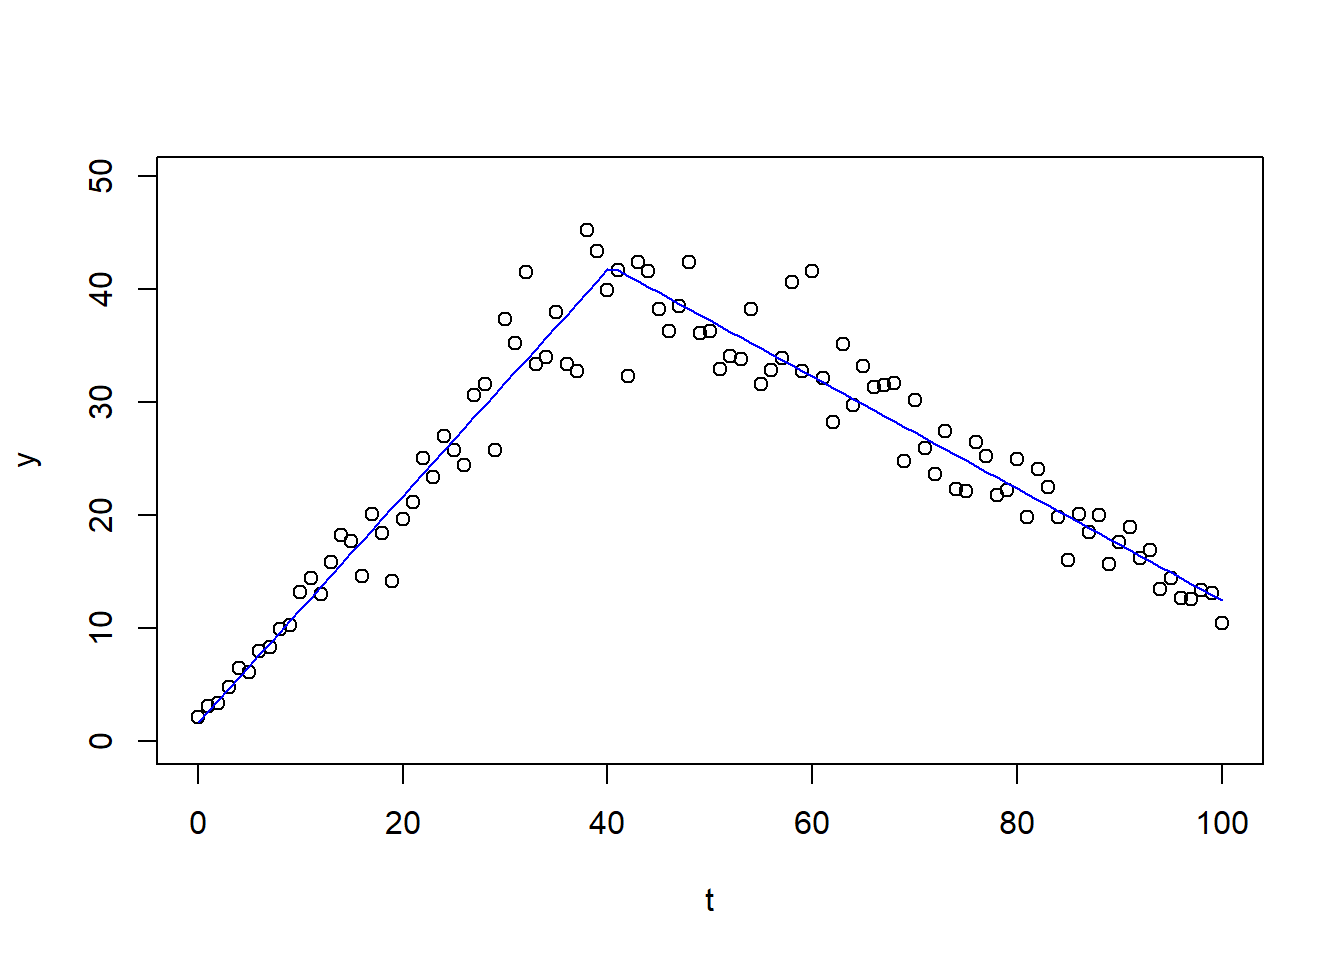
\includegraphics{20230905_twoLine_model_files/figure-latex/unnamed-chunk-1-1.pdf}

\end{document}
